\chapter{Implementation}
\label{sec:implementation}

Isharati is a full-stack web application built from three separately hosted parts: the \emph{data} (corpora, retrieval
embeddings, sign lexicons with their poses) are a versioned dataset on the Hugging Face Hub; the \emph{language models}
are reached through OpenRouter; and the \emph{application} (the pipeline API and the web interface) runs as a Docker
container on a Hugging Face Space (Figure~\ref{fig:impl}). The container holds code and configuration only; everything
else is fetched at start-up and at request time with authenticated API calls.

\begin{figure}[ht]
\centering
\resizebox{\textwidth}{!}{%
\begin{tikzpicture}[node distance=6mm and 9mm,
  box/.style={draw=navy, rounded corners=2pt, fill=soft, align=center, font=\small, text width=36mm, minimum height=13mm},
  hub/.style={draw=amberx!90!black, fill=amberx!12, align=center, font=\small, text width=36mm, minimum height=13mm},
  arr/.style={-{Stealth[length=2mm]}, thick, navy}]
  \node[box] (web) {\textbf{Browser}\\question, cited answer,\\gloss chips, avatar\\(three.js + VRM)};
  \node[box, right=of web] (fn) {\textbf{Hugging Face Space}\\Docker: FastAPI pipeline\\and web interface};
  \node[hub, right=of fn] (or) {\textbf{OpenRouter}\\one API, many models;\\first model per task,\\fallbacks behind it};
  \node[hub, below=10mm of fn] (hf) {\textbf{Hub dataset}\\\code{isharati-data}: en, ar,\\tr, ur folders (private)};
  \node[hub, below=10mm of or] (embapi) {\textbf{HF inference}\\multilingual E5-large\\for the question};
  \draw[arr] (web) -- node[above, font=\scriptsize]{HTTPS} (fn);
  \draw[arr] (fn) -- node[above, font=\scriptsize]{LLM calls} (or);
  \draw[arr] (hf) -- node[left, font=\scriptsize, align=right]{token-\\authenticated\\download} (fn);
  \draw[arr] (fn) -- (embapi);
\end{tikzpicture}}
\caption{Deployment: the dataset on the Hugging Face Hub, language models through OpenRouter, the application as a
Docker Space.}
\label{fig:impl}
\end{figure}

\section{Data layer: the Hugging Face dataset}
All data the application reads is one private dataset on the Hub, organised by language (Table~\ref{tab:hubdata}). Each
language folder holds the Qur'an and hadith corpus of that language (\code{corpus.jsonl}, the format of
Section~\ref{sec:textdata}), its E5 passage embeddings with their passage identifiers, its sign lexicon table(s), and the
poses of the signs in one compressed archive per lexicon; the Arabic folder also holds the cached CAMeL lemmas of the
corpus words and the back-translation templates. A \code{layout.json} file maps every file to the path the pipeline
expects, so the same code runs in development and on the Space. The dataset card documents the fields, the pose format,
the sources and their licences, and declares one viewer configuration per corpus and per lexicon.

\begin{table}[ht]
\centering\small
\caption{The Hub dataset, one folder per language (1.1\,GB in total).}
\label{tab:hubdata}
\begin{tabular}{l l l r r r}
\toprule
Folder & Text & Sign language & Passages (Qur'an / hadith) & Glosses & Signs with poses \\
\midrule
\code{en/} & English & ASL & 8,564 (6,236 / 2,328) & 3,055 & 3,011 \\
\code{ar/} & Arabic & ArSL & 9,810 (6,236 / 3,574) & 3,979 & 3,755 \\
\code{tr/} & Turkish & T\.{I}D & 8,386 (6,236 / 2,150) & 1,136 & 1,308 \\
\code{ur/} & Urdu & ISL & 8,456 (6,236 / 2,220) & 6,411 & 8,021 \\
\bottomrule
\end{tabular}
\end{table}

Each dataset revision is immutable, so every answer is reproducible: a new sign or a corrected corpus takes effect when a
new revision is published. The dataset is private because several sign sources do not permit redistribution
(Chapter~\ref{sec:statements}); the Space reads it with a Hugging Face access token stored as a Space secret, and the
browser never receives more than the pose of one answer.

\section{Model layer: OpenRouter and hosted embeddings}
All language-model calls go through OpenRouter's OpenAI-compatible API with one key, stored as a Space secret. The models
are an ordered list: Qwen 3.8 27B first, then Nemotron 3 Ultra and Nemotron 3 Super (Table~\ref{tab:llms}), all on
OpenRouter's free tier; the next model is tried when one times out, is rate-limited, or returns its reasoning instead of an
answer. Reasoning output is switched off in every request. The order was set by a comparison on held-out ArabSign
sentences, where Qwen gave a lower gloss error than Nemotron; because grounding is enforced by checks on the output and not
by the model, models can be replaced without weakening the guarantees, and the list is a setting of the Space. The question
is embedded by Hugging Face hosted inference of the same multilingual E5 model that embedded the passages; we verified that
hosted and local vectors are identical (cosine similarity 1.0), so the stored passage embeddings are used unchanged. BM25
remains the fallback if the embedding call fails.

\section{Application layer: the Docker Space}
The Space runs a Python container (FastAPI server and the single-page interface on one port). At start-up it downloads the
dataset revision for the configured languages (English and Arabic), restores the data layout and unpacks the poses, which
takes under half a minute; a marker per revision makes later restarts skip this. The pipeline of
Chapter~\ref{sec:architecture} then runs per request: referral check, hybrid retrieval, grounded answer, glossing, pose
assembly, skeleton video, and the per-word report.

\begin{table}[ht]
\centering\small
\caption{HTTP interface of the application.}
\label{tab:api}
\begin{tabularx}{\textwidth}{L{3.6cm} Y}
\toprule
Route & Returns \\
\midrule
\code{POST /api/ask} & for a question and a language (\code{en} or \code{ar}): status (signed, referred or unanswered),
answer, sources with links, glosses, missing signs, coverage, per-word trace, back-translation score, sign segments with
times, and the run identifier \\
\code{GET /pose/\{id\}.json} & the assembled pose of a run ($T\times 50\times 3$ at 25\,fps), which drives the avatar \\
\code{GET /video/\{id\}.mp4} & the skeleton video of a run \\
\code{GET /api/avatars} & the VRM avatar models available \\
\code{GET /static/\{name\}} & the avatar model, the retargeting and outfit code \\
\bottomrule
\end{tabularx}
\end{table}

The interface is a single page in English and Arabic (right-to-left): the question box with example questions, the cited
answer with links to its sources, gloss chips highlighted while signed (missing signs in red), and the player with the
avatar or skeleton view, the outfit panel, the speed selector and video export. The avatar is rendered in the browser from
the pose with three.js and three-vrm.

\begin{table}[ht]
\centering\small
\caption{Components and the services that host them.}
\label{tab:stack}
\begin{tabularx}{\textwidth}{L{3.4cm} L{3.4cm} Y}
\toprule
Component & Service & Role \\
\midrule
Corpora, embeddings, lexicons, poses & Hugging Face dataset & versioned, private, organised by language; token access \\
Language models & OpenRouter & ordered model list with fallbacks, one key \\
Question embedding & Hugging Face inference & multilingual E5-large, identical to the passage index \\
Pipeline and interface & Hugging Face Docker Space & FastAPI server, skeleton video, web page \\
3D Avatars \& VRM assets & Space static assets & 6 rigged VRM 1.0 humanoid models (Rocketbox + Pixiv) \\
Secrets & Space settings & Hugging Face token, OpenRouter key \\
\bottomrule
\end{tabularx}
\end{table}

\section{3D avatar assets and runtime rendering pipeline}
\label{sec:avatars}
To provide natural, engaging sign language production beyond 2D stick-figure skeletons, Isharati incorporates a full WebGL-based 3D humanoid avatar engine. The system supports six distinct avatars (Figure~\ref{fig:avatar_roster} and Table~\ref{tab:avatar_roster}) that sign in real time inside the browser without requiring server-side video rendering.

\begin{figure}[ht]
\centering
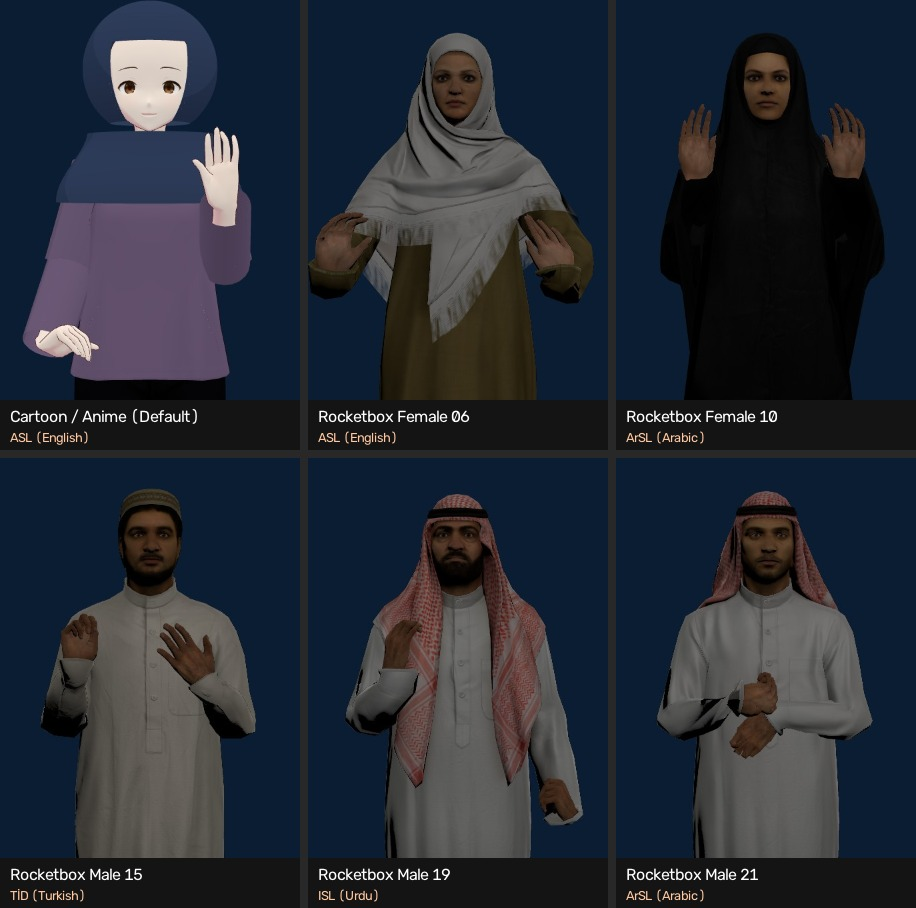
\includegraphics[width=\textwidth,height=0.48\textheight,keepaspectratio]{figures/avatar_roster.jpg}
\caption{The six 3D humanoid avatars available in Isharati, each shown signing a sample Qur'anic/hadith gloss in their corresponding language mode. Top row: Cartoon/Anime default (ASL, ``PEACE''), Rocketbox Female 06 (ASL, ``PRAYER''), Rocketbox Female 10 (ArSL, ``ALLAH''). Bottom row: Rocketbox Male 15 (T\.{I}D, ``BARI\c{S}''), Rocketbox Male 19 (ISL, ``MOSQUE''), Rocketbox Male 21 (ArSL, ``ZAKAH''). All avatars support modest dress presets (hijab, shemagh, and traditional thobe).}
\label{fig:avatar_roster}
\end{figure}

\subsection{Avatar asset provenance and licensing}
The platform incorporates two categories of humanoid meshes:
\begin{enumerate}[leftmargin=*,itemsep=2pt]
  \item \textbf{Stylized / Anime default (\texttt{avatar.vrm}):} Based on Pixiv's official sample model (\texttt{VRM1\_Constraint\_Twist\_Sample}), distributed under an open MIT-equivalent license permitting modification, commercial use, and religious application without attribution (\url{https://github.com/vrm-c/vrm-specification}). It serves as a lightweight, universal baseline ($10.8$\,MB).
  \item \textbf{Photorealistic adult humanoids (\texttt{rocketbox\_*.vrm}):} Derived from the \textbf{Microsoft Rocketbox Avatar Library} \cite{rocketbox}, an open-source library of rigged adult characters released by Microsoft Research under the permissive MIT License (\url{https://github.com/microsoft/Microsoft-Rocketbox}). Five diverse character archetypes were selected to represent different cultural demographics across the four supported language communities (Table~\ref{tab:avatar_roster}).
\end{enumerate}

\begin{table}[ht]
\centering\small
\caption{The six production 3D humanoid avatars in Isharati.}
\label{tab:avatar_roster}
\begin{tabularx}{\textwidth}{L{3.2cm} L{1.8cm} L{1.5cm} L{1.6cm} r r Y}
\toprule
Model ID & Demographic & Lang. & Sign Lang. & Size & Vertices & Primary Preset \\
\midrule
\texttt{avatar.vrm} & Stylized / Anime & \code{en} & ASL & 10.8\,MB & 21,432 & Modest tunic + hijab \\
\texttt{rocketbox\_female\_06} & Adult Female & \code{en} & ASL & 6.2\,MB & 18,720 & Long dress + hijab drape \\
\texttt{rocketbox\_female\_10} & Adult Female & \code{ar} & ArSL & 3.5\,MB & 16,944 & Black abaya + hijab \\
\texttt{rocketbox\_male\_15} & Adult Male & \code{tr} & T\.{I}D & 5.5\,MB & 19,102 & White thobe + kufi cap \\
\texttt{rocketbox\_male\_19} & Adult Male & \code{ur} & ISL & 5.3\,MB & 18,850 & White thobe + shemagh \\
\texttt{rocketbox\_male\_21} & Adult Male & \code{ar} & ArSL & 6.0\,MB & 19,340 & White thobe + shemagh \\
\bottomrule
\end{tabularx}
\end{table}

\subsection{Automated Blender conversion pipeline (\texttt{rocketbox\_to\_vrm.py})}
The raw Rocketbox assets are distributed as Autodesk 3ds Max FBX files with 3ds Max Biped armatures and uncompressed 2048$\times$2048 TGA textures. Because web-based sign language animation requires fast mobile downloads and strict compliance with the modern VRM 1.0 standard \cite{vrm}, we engineered a headless, automated conversion pipeline using Blender 4 and the official VRM Add-on for Blender (\url{https://github.com/saturday06/VRM_Addon_for_Blender}). The automated conversion script (\texttt{scripts/avatars/rocketbox\_to\_vrm.py}) executes five major preprocessing stages:

\paragraph{1. Texture optimization and channel re-wiring.} Raw textures are extracted from TGA archives, downsampled from 2048\,px to 1024\,px, and compressed into web-optimized PNGs. Specular maps (which lack standard glTF PBR material slots) are stripped to reduce payload size. For hair, eyelashes, and semi-transparent fabrics, the texture's alpha channel is connected to the Principled BSDF's alpha input with hashed transparency (\texttt{HASHED} alpha blend mode) to prevent sorting artifacts. This reduces the raw texture payload from over 45\,MB to under 5\,MB per avatar.

\paragraph{2. Armature hierarchy correction.} In 3ds Max Biped rigs, the thigh bones (\texttt{Bip01 L/R Thigh}) are parented directly to the pelvis/spine, and the clavicles (\texttt{Bip01 L/R Clavicle}) are parented to the neck bone. The VRM 1.0 humanoid specification strictly requires leg bones under the hips/pelvis and clavicles under \texttt{Spine2} (the upper chest). The script programmatically enters armature edit mode and re-parents these bone joints into the valid humanoid tree, preserving skinning weights and vertex deformation invariants.

\paragraph{3. Humanoid bone retargeting and finger rigging.} The script maps all 55 standard humanoid joints, including full 3-segment finger articulation for all five digits on each hand: thumb (\texttt{Finger0}, \texttt{01}, \texttt{02}), index (\texttt{Finger1}, \texttt{11}, \texttt{12}), middle (\texttt{Finger2}, \texttt{21}, \texttt{22}), ring (\texttt{Finger3}, \texttt{31}, \texttt{32}), and little finger (\texttt{Finger4}, \texttt{41}, \texttt{42}). This fine finger topology is essential for conveying the intricate manual phonology of sign languages.

\paragraph{4. Scale normalization and rest-pose stabilization.} 3ds Max exports in centimeter units with a 0.01 armature scale. The script applies all object transforms, normalizes the root to SI meters, and bakes the geometry. The native Rocketbox A-pose is deliberately preserved as the rest orientation rather than forced into a T-pose, avoiding the distortion or destruction of the 176 facial blendshapes/shape keys stored in the original mesh.

\paragraph{5. VRM 1.0 metadata serialization.} Compliant VRM 1.0 headers are written, explicitly encoding title, author attribution (``Microsoft Rocketbox''), MIT license references, and permissible usage flags (commercial use, modification, and religious/educational usage all enabled).

\subsection{Client-side kinematic retargeting (\texttt{avatar.js})}
Inside the browser, the avatar is loaded via three.js \cite{threejs} and the \texttt{@pixiv/three-vrm} library \cite{threevrm}. Every frame, the continuous MediaPipe $[50, 3]$ coordinate stream is converted into bone rotations in real time:

\paragraph{Bone direction vectors.} For each limb segment (upper arm, lower arm), the rest-pose direction vector is measured from the avatar's initial skeletal rest state. The rotation quaternion between the rest vector and the incoming MediaPipe joint displacement vector is computed using spherical vector projection.

\paragraph{Palm orientation recovery.} MediaPipe returns 21 3D points per hand. The normal of the hand plane is constructed from the cross-product of the wrist-to-middle-knuckle vector and the index-knuckle-to-pinky-knuckle vector:
\begin{equation}
  \mathbf{v}_{\text{long}} = \mathbf{p}_{\text{middle}} - \mathbf{p}_{\text{wrist}}, \quad
  \mathbf{v}_{\text{lat}} = \mathbf{p}_{\text{pinky}} - \mathbf{p}_{\text{index}}, \quad
  \mathbf{n}_{\text{palm}} = \mathbf{v}_{\text{long}} \times \mathbf{v}_{\text{lat}}.
\end{equation}
This recovers the exact 3D orientation of the palm (facing inward, outward, upward, or downward) across complex signing motions.

\paragraph{Finger flexion retargeting.} Each finger's proximal, intermediate, and distal joints are rotated based on the angle between adjacent phalange vectors, allowing the avatar to produce crisp handshapes (e.g., fists, flat hands, pointing fingers).

\paragraph{Anatomical stability guards.} Raw monocular MediaPipe depth ($z$-axis) is noisy. We dampen depth fluctuations by 50\%, enforce non-penetration constraints preventing the hands from clipping into the torso mesh, and apply an exponential moving average ($\alpha{=}0.55$) over joint quaternions to eliminate high-frequency visual jitter.

\subsection{Procedural modesty presets (\texttt{outfits.js})}
To ensure that all generated animations remain culturally and religiously respectful across Islamic educational and religious settings, Isharati implements a procedural modesty subsystem (\texttt{outfits.js}). Rather than requiring separate 3D models for every clothing style, modesty elements are procedurally constructed in WebGL:

\paragraph{Hijab preset.} Generates a tight-fitting head undercap and a graceful draped mantle over the neck and upper chest, bound to the \texttt{Head}, \texttt{Neck}, and \texttt{UpperChest} bones. Sleeves are procedurally extended to the wrists if the base model has short sleeves.

\paragraph{Shemagh / Ghutrah preset.} Generates a traditional Arabian folded headdress with an \emph{agal} (black headband), draped over both shoulders. The underlying shirt/trousers are dynamically shaded with a white matte material to represent a traditional Arabian \emph{thobe}.

\paragraph{Dynamic geometry fitting.} Because all six avatars have differing cranial circumferences and shoulder widths, the outfit generator measures the distance between the avatar's eye bones and temple vertices at load time, dynamically scaling the mesh offsets so that the hijab and shemagh fit any avatar without clipping or gaps.

Users can toggle between presets, customize fabric colors, adjust playback speeds ($0.5\times$ to $1.25\times$), and export rendered signing animations as WebM/MP4 clips directly from the browser.

\section{Development and evaluation setup}
The pipeline code is the same in development, where it runs as a local server with the data on disk, a local GPU
embedding service and NVIDIA NIM with a Groq fallback as model providers (Table~\ref{tab:llms}). 198 automated tests cover
the normalisation and matching rules, the grounding checks, the pose assembly, the model-client selection and the
restoration of the data from the Hub. All measurements in Chapters~\ref{sec:eda} and~\ref{sec:results} were taken in the
development setup with the models of Table~\ref{tab:llms}.
